\documentclass[fleqn]{jbook}
\usepackage{physpub}

\begin{document}

\begin{question}{専攻 問題7}{}

% Definition of local macros

生物の身体はしばしば左右非対称性を示す。見かけ上対称な受精卵から
発生する個体が非対称となる分子機構はまだほとんど理解されていない。
しかし、ある巻き貝(Limneae)が右巻き型になるか左巻き型になるかは
一つの遺伝子の2種の対立遺伝子(S:左巻き型、s:右巻き型)で決まること
が知られている。\\
下に説明する 実験(1) と 実験(2) の結論をよく読んで、
下記の3つの問に答えなさい。\\

\leftline{\bf 実験(1)}
\begin{list}{}{\itemindent=0mm \topsep=0mm}
\item[] 右巻き型と左巻き型の発生における左右非対称性は、下図に描かれて
        いるように、第2回目の細胞分裂に始まり、それ以後の発生は鏡像
        対称的に進行する。第2分裂の頃にはまだ受精卵の染色体からの
        メッセンジャーRNA (mRNA)の合成は全く行われていない。 
        (図中のABCなどは分裂した細胞につけられた名前である)
\end{list}

\begin{center}
\mbox{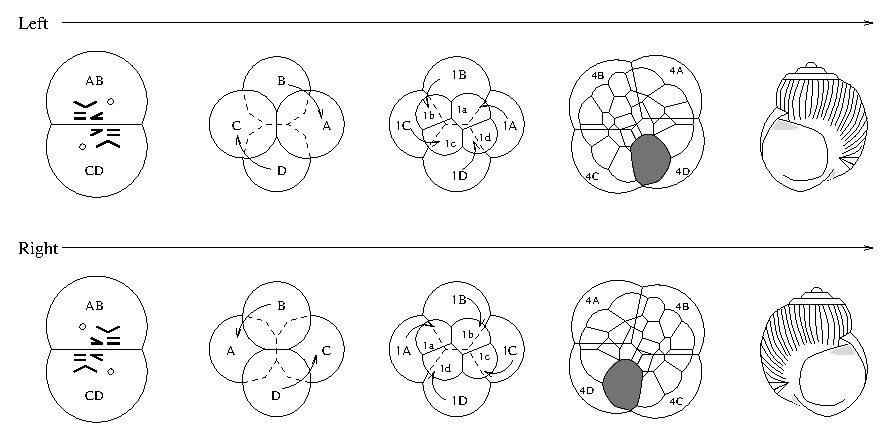
\includegraphics[clip]{1996phy7-1.eps}}
\end{center}

\leftline{\bf 実験(2)}
\begin{list}{}{\itemindent=0mm \topsep=0mm \itemsep=0mm \parsep=0mm}
\item[\bf 1)]
  純系右巻き(s/s)の雄個体と純系左巻き(S/S)雌個体との交配をしたら、
  その第1世代(F1)は全個体が左巻きであった。

\item[\bf 2)]
  そのF1雌雄を交配してできた第2世代(F2)は全個体が左巻きであった。

\item[\bf 3)]
  そのF2雌雄を交配してできた第3世代(F3)には右巻きと左巻きの個体が
  混在し、その比はおよそ 1:3 であった。
\end{list}


\begin{subquestions}
\SubQuestion
  実験(2)の結果は、明確な遺伝現象ではあるがメンデルの法則にはあわない
  変則的なもののように見える。しかし実験(1)の結果を吟味して考えると、
  メンデルの法則で完全に理解できることを説明せよ。

\SubQuestion
  実験(2)とは逆に、純系左巻き(S/S)雄と純系右巻き(s/s)雌とを交配した
  場合、そのF1、F2、F3個体の巻き方はどのようになるかを推論しなさい。

\SubQuestion
  非対称性生成の分子機構を明らかにするためには、この遺伝子の産物
  (メッセンジャーRNAおよび蛋白質)についてどのような研究をするべきかを
  箇条書きにして論じ、S遺伝子産物の働きについてどのような可能性がある
  かを論じなさい。

\end{subquestions}
\end{question}
\begin{answer}{専攻 問題7}{}

\begin{subanswers}
\SubAnswer
  \parbox[t]{80mm}{
  {\bf[解答例1]}\\
  実験(2)では、子の巻き方は母貝の遺伝子型に対応している。
  (これがポイント、もちろんメンデルの法則に対応)
  これは実験(1)の結果の、左右非対称型が決定する時点で受精卵の
  染色体からのmRNAの合成が全く行われていないことに対応している。
  つまり、左右非対称性は卵中にある母貝由来の物質によって
  決定されていると考えられる。

  {\bf[解答例2]}\\
  実験(1)より、右巻き型と左巻き型の分化は第二分裂に始まるので、
  核中の遺伝子の情報の影響を受けて分化したのではないことがわかる。
  つまりこの遺伝現象は、子にそのまま引き継がれる卵細胞の細胞質に
  より子の形質が決定される細胞質遺伝である。そのため、母親の遺伝子
  が示す形質が母親では発現せず、1世代遅れて次の代で現れる。
  よって実験(2)の結果が完全に理解できる。


\SubAnswer
  F1では母親が右巻き純系であるので右巻きになる。
  F2では母親(F1)が S/s であるので優性の左巻きになる。
  F3では同様に母親の遺伝型があらわれ、
  右巻きと左巻きが $1:3$ になる。\\
  }\parbox[t]{75mm}{\vspace*{-10mm}
  \begin{center}
    \mbox{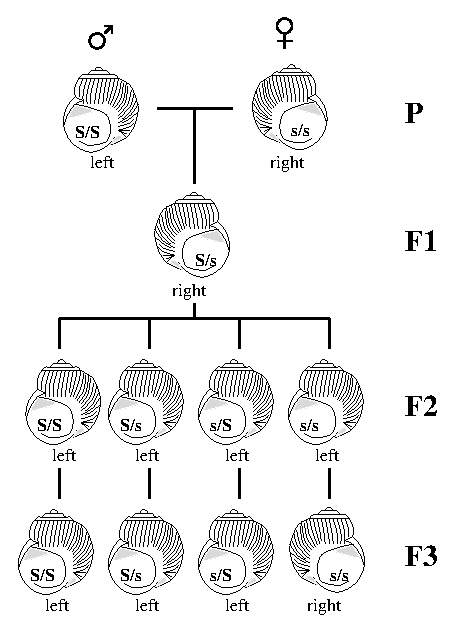
\includegraphics[clip]{1996phy7-2.eps}}\\
    巻貝の家系図
  \end{center}}



\SubAnswer
  \begin{itemize}
  \item
    Sタンパク質のアッセイ系の確立
  \item
    Sタンパク質の単離
  \item
    S遺伝子の塩基配列の決定
  \item
    S遺伝子をベクターに組み込み、純系右巻きになる予定の卵に
    導入し、その個体が左巻きになるかみる。
  \item 
    この遺伝子により作られたタンパク質が、細胞分裂の際どのように
    回転方向を決定し回転を作っているのか調べる。
  \item
    受精の後、しばらく m-RNA が作られないが、m-RNA の製造を止める
    情報がこの遺伝子に書かれているのか調べる。
  \item
    大腸菌などで、Sタンパク質を大量に発現させSタンパク質の
    抗体を作る。
  \item
    大量に抗体を注射すると、抗体がSタンパク質に結合すること
    によってSタンパク質の働きが阻害されるかもしれない。
    それによって起こる現象を観察する。
  \item
    活性をもたせたまま蛍光物質を結合させたSタンパク質を作成し、
    それを卵に注射する。それを蛍光顕微鏡でみると卵中のどこで
    Sタンパク質が作用しているかがわかる。
  \item
    Sタンパク質によって影響を受ける物質を探索する。
  \item
    Sタンパク質の構造を、X線結晶解析、NMRで決定し、構造から
    Sタンパク質の機能を推定する。
  \end{itemize}

  S遺伝子産物の働きは、細胞分裂時に細胞質分裂に影響を与える
  (特に細胞骨格など)タンパクじゃないかと私は考えるんですが、
  細胞周期に関係するかもしれませんし、ぜんぜん違うかもしれません。
  上にずらずら並べた実験の結果をみないとなんとも言えません。
  論じろっていわれても結構困るかも。

\end{subanswers}
\end{answer}


\end{document}
